\documentclass[pdflatex,compress,mathserif]{beamer}

%\usetheme[dark,framenumber,totalframenumber]{ElektroITK}
\usetheme[darktitle,framenumber,totalframenumber]{ElektroITK}

\usepackage[utf8]{inputenc}
\usepackage[T1]{fontenc}
\usepackage{lmodern}
\usepackage[bahasai]{babel}
\usepackage{amsmath}
\usepackage{amsfonts}
\usepackage{amssymb}
\usepackage{graphicx}
\usepackage{multicol}

\newcommand*{\Scale}[2][4]{\scalebox{#1}{$#2$}}%

\title{PEMODELAN JARINGAN KOMUNIKASI}
\subtitle{STP - Spanning Tree Protocol}

\author{Tim Dosen Pengampu}

\begin{document}
	
\maketitle

\section{Layer 3 Path Selection and Loop Prevention Review}

\begin{frame}
	\frametitle{Layer 3 Network Redundancy Review}
	\begin{multicols}{2}
		\begin{center}
			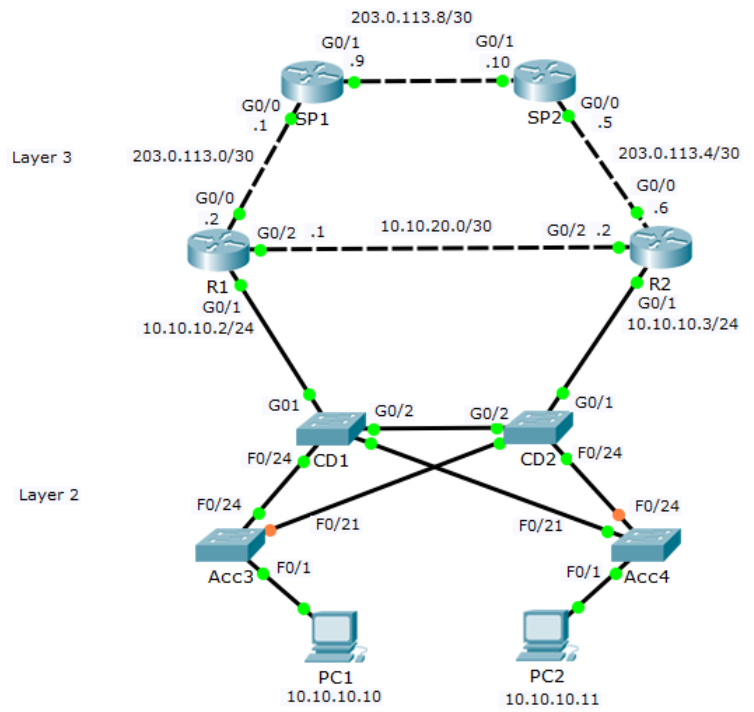
\includegraphics[width=\linewidth]{img/img01}
		\end{center}
		\columnbreak
		\begin{itemize}
			\item Layer 3 routing and HSRP control the
path selection and provide automatic
failover for Layer 3 connections
		\end{itemize}
	\end{multicols}
\end{frame}

\begin{frame}
	\frametitle{Layer 3 Network Redundancy Review}
	\begin{multicols}{2}
		\begin{center}
			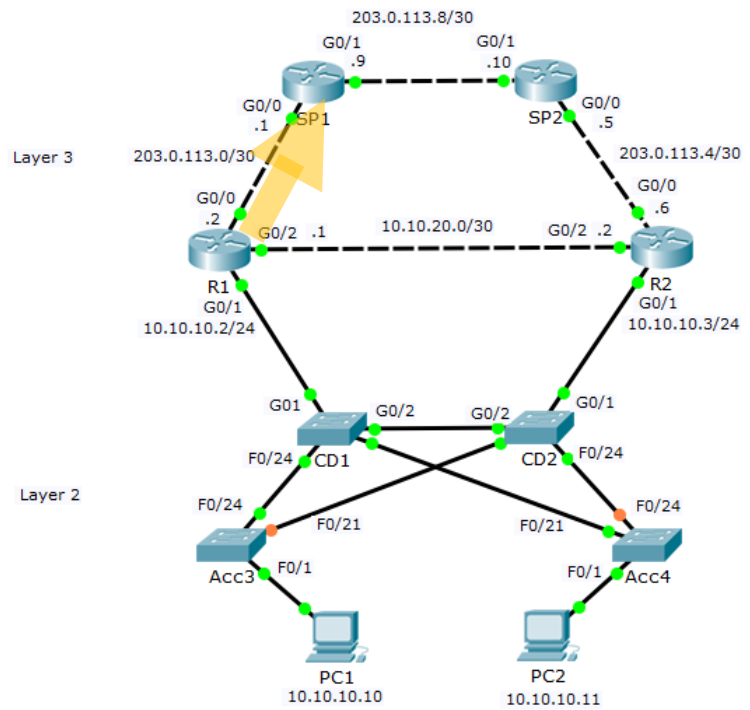
\includegraphics[width=\linewidth]{img/img02}
		\end{center}
		\columnbreak
		\begin{itemize}
			\item Routes on R1:
		\end{itemize}
		\begin{center}
			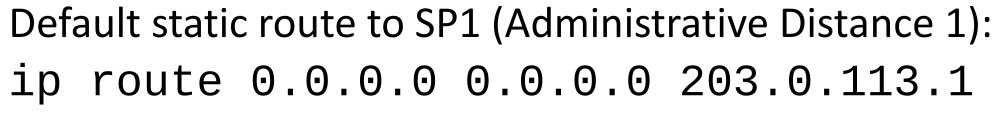
\includegraphics[width=\linewidth]{img/img03}
		\end{center}
	\end{multicols}
\end{frame}

\begin{frame}
	\frametitle{Network Redundancy – Layer 3 Configuration}
	\begin{multicols}{2}
		\begin{center}
			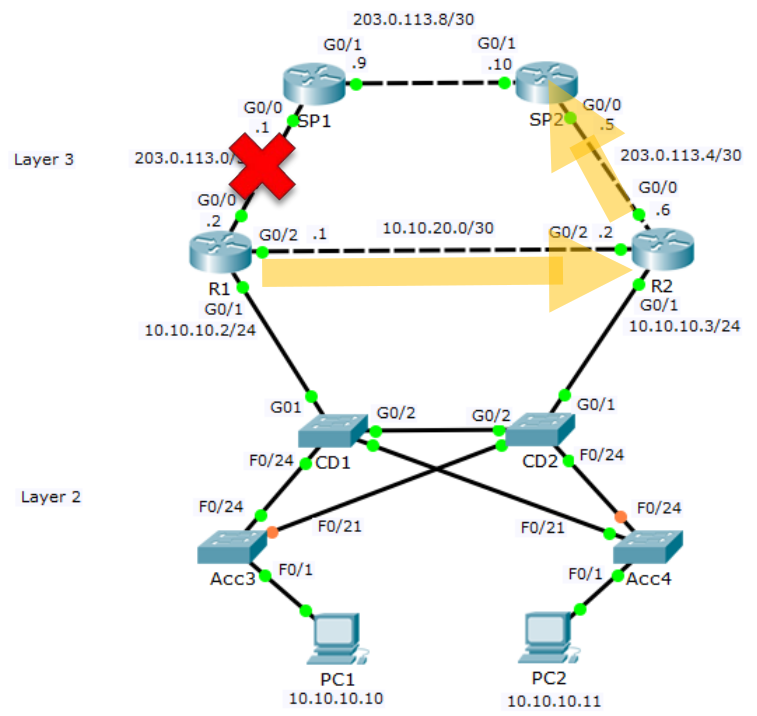
\includegraphics[width=\linewidth]{img/img04}
		\end{center}
		\columnbreak
		\begin{itemize}
			\item Routes on R1:
		\end{itemize}
		\begin{center}
			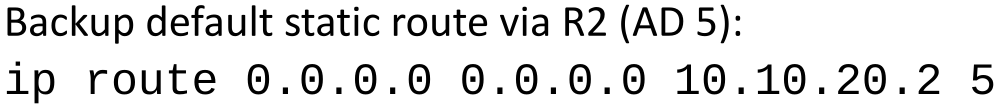
\includegraphics[width=\linewidth]{img/img05}
		\end{center}
	\end{multicols}
\end{frame}

\begin{frame}{Network Redundancy – Layer 3 Configuration}
	\begin{multicols}{2}
		\begin{center}
			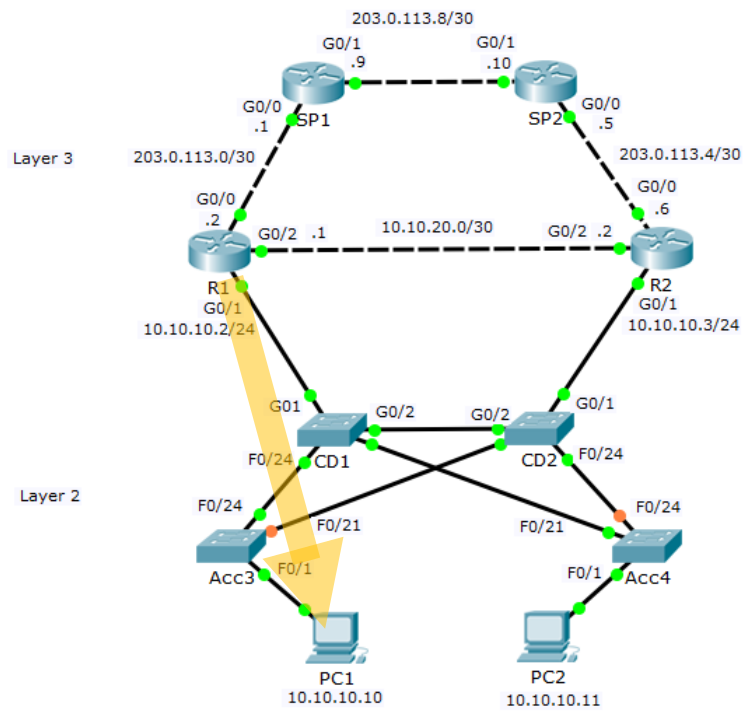
\includegraphics[width=\linewidth]{img/img06}
		\end{center}
		\columnbreak
		\begin{itemize}
			\item Routes on R1:
		\end{itemize}
		\begin{center}
			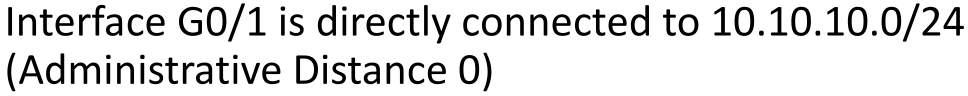
\includegraphics[width=\linewidth]{img/img07}
		\end{center}
	\end{multicols}
\end{frame}

\begin{frame}{Network Redundancy – Layer 3 Configuration}
	\begin{multicols}{2}
		\begin{center}
			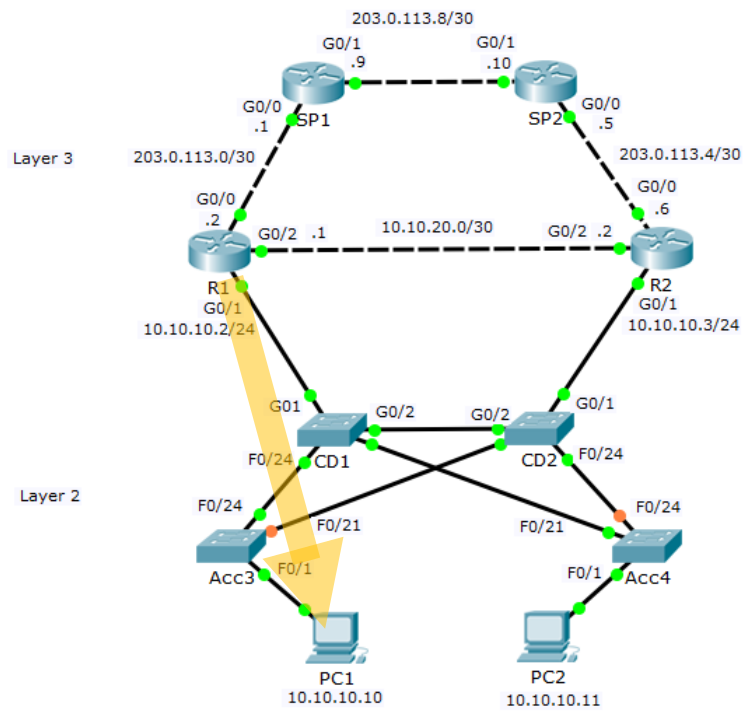
\includegraphics[width=\linewidth]{img/img06}
		\end{center}
		\columnbreak
		\begin{itemize}
			\item Routes on R1:
		\end{itemize}
		\begin{center}
			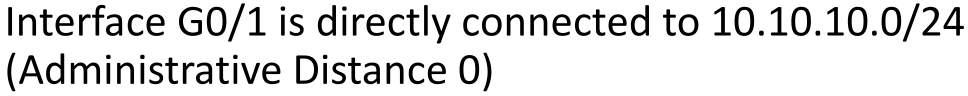
\includegraphics[width=\linewidth]{img/img07}
		\end{center}
	\end{multicols}
\end{frame}

\begin{frame}{Network Redundancy – Layer 3 Configuration}
	\begin{multicols}{2}
		\begin{center}
			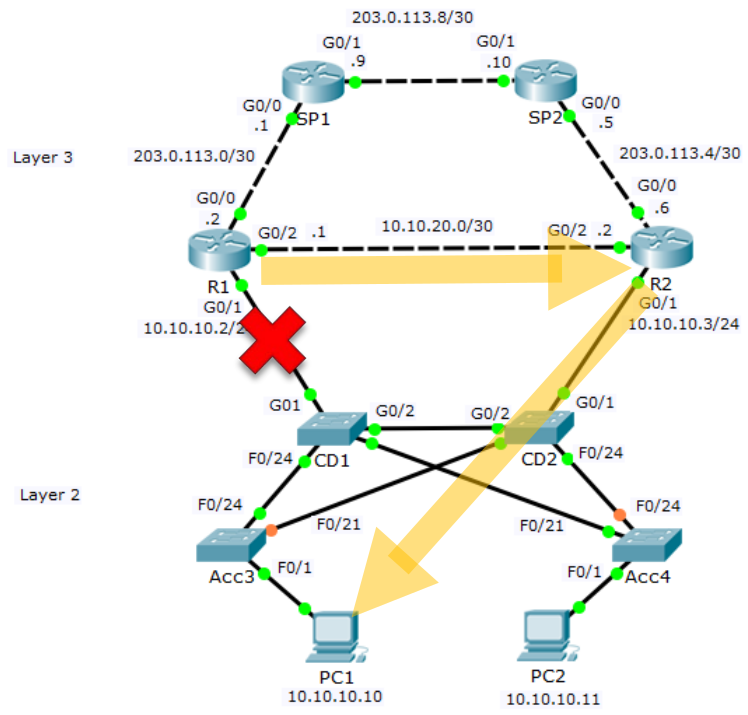
\includegraphics[width=\linewidth]{img/img08}
		\end{center}
		\columnbreak
		\begin{itemize}
			\item Routes on R1:
		\end{itemize}
		\begin{center}
			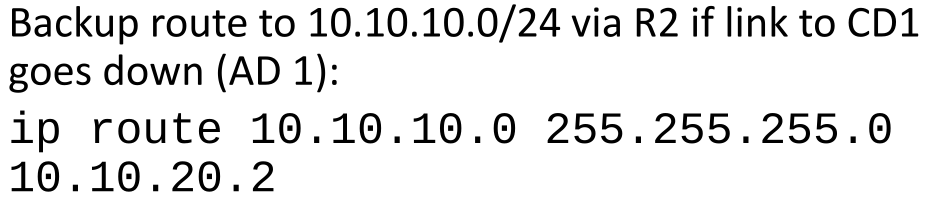
\includegraphics[width=\linewidth]{img/img09}
		\end{center}
	\end{multicols}
\end{frame}

\begin{frame}
	\frametitle{HSRP Hot Standby Router Protocol}
	\begin{multicols}{2}
		\begin{center}
			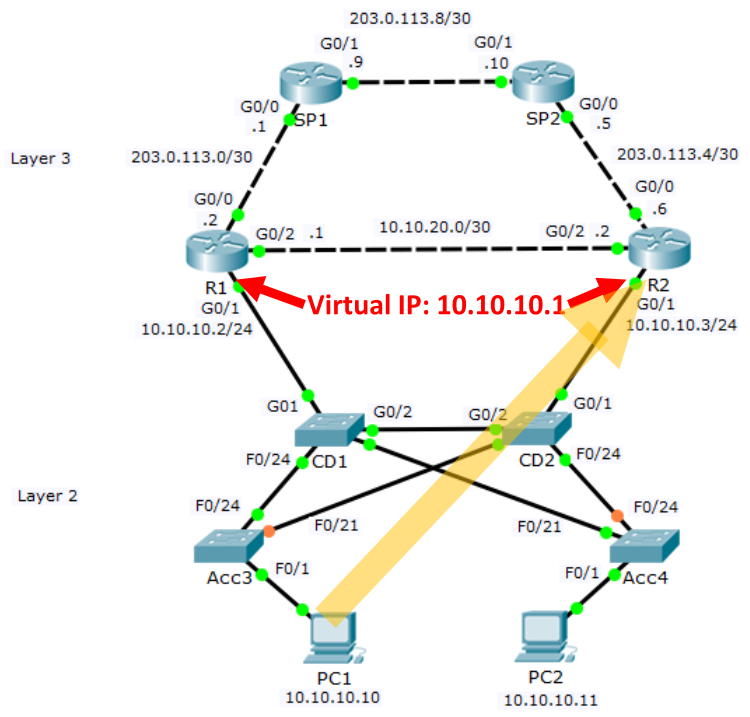
\includegraphics[width=\linewidth]{img/img10}
		\end{center}
		\columnbreak
		\begin{center}
			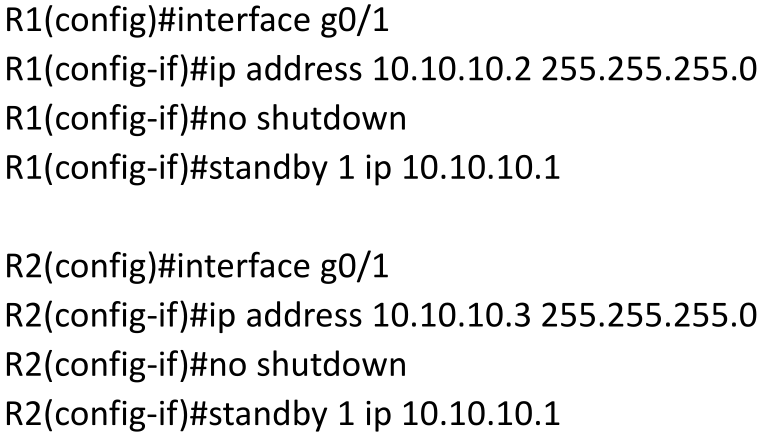
\includegraphics[width=\linewidth]{img/img11}
		\end{center}
	\end{multicols}
\end{frame}

\begin{frame}{HSRP Hot Standby Router Protocol}
	\begin{multicols}{2}
		\begin{center}
			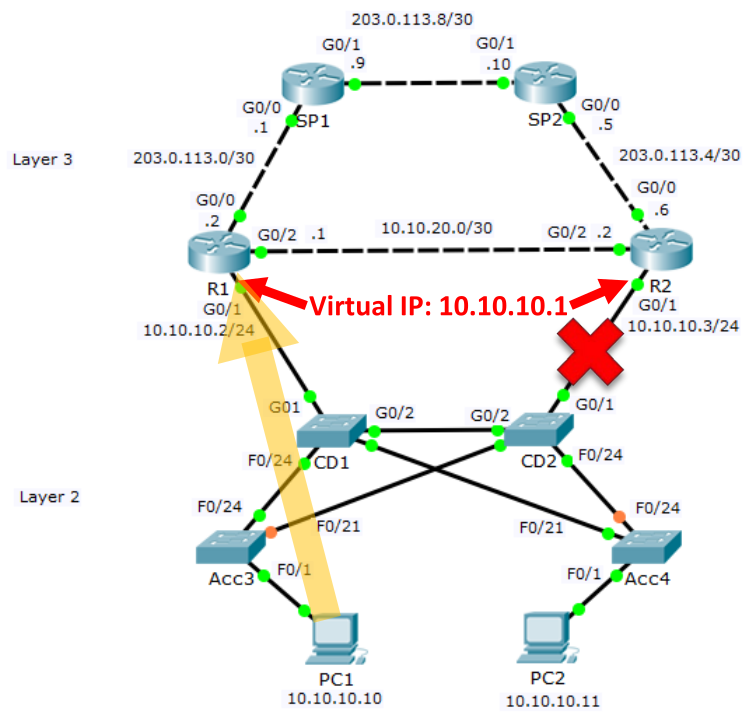
\includegraphics[width=\linewidth]{img/img12}
		\end{center}
		\columnbreak
		\begin{center}
			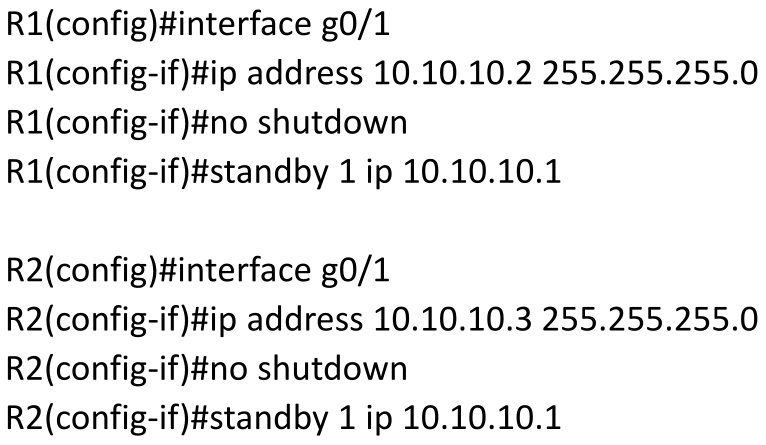
\includegraphics[width=\linewidth]{img/img13}
		\end{center}
	\end{multicols}
\end{frame}

\begin{frame}
	\frametitle{Routing Loop}
	\begin{multicols}{2}
		\begin{center}
			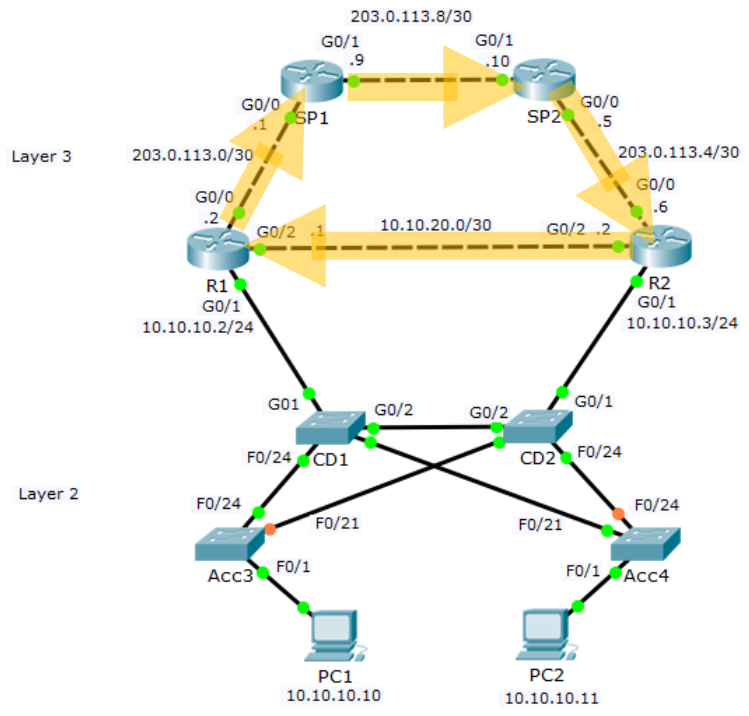
\includegraphics[width=\linewidth]{img/img14}
		\end{center}
		\columnbreak
		\begin{center}
			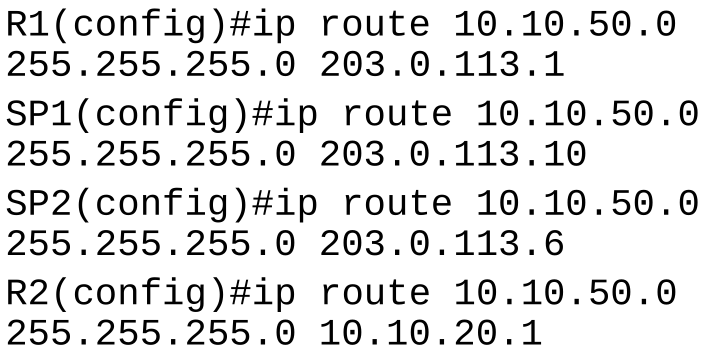
\includegraphics[width=\linewidth]{img/img15}
		\end{center}
	\end{multicols}
\end{frame}

\begin{frame}
	\frametitle{The IP Header Time to Live Field}
	\begin{center}
		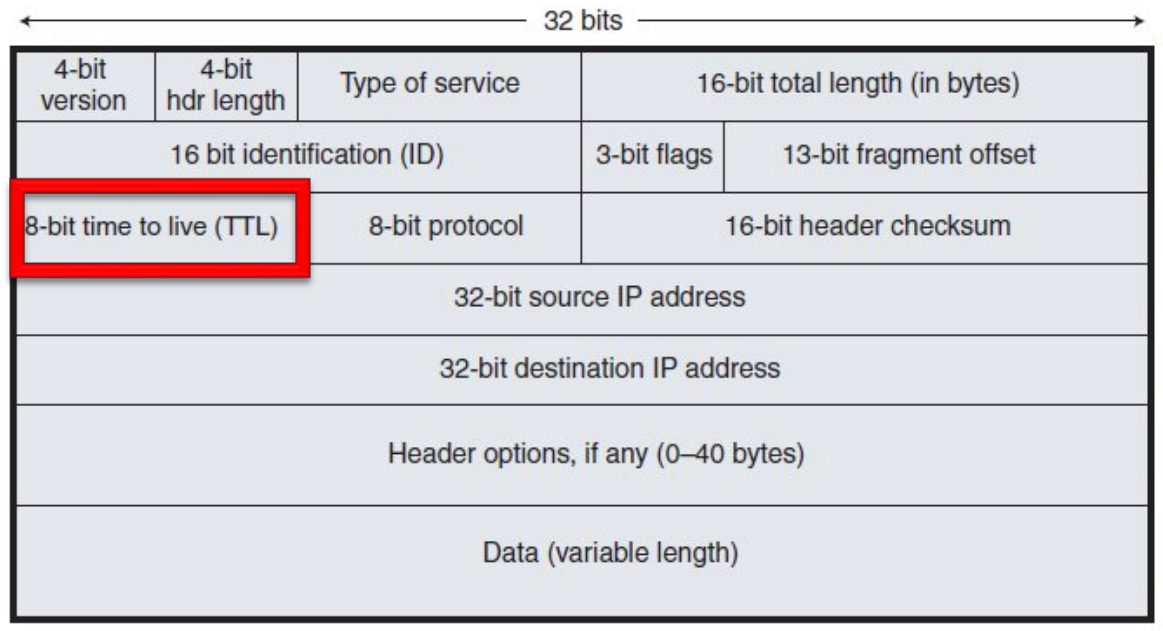
\includegraphics[width=\linewidth]{img/img16}
	\end{center}
\end{frame}

\begin{frame}
	\frametitle{Routing Loop}
	\begin{center}
		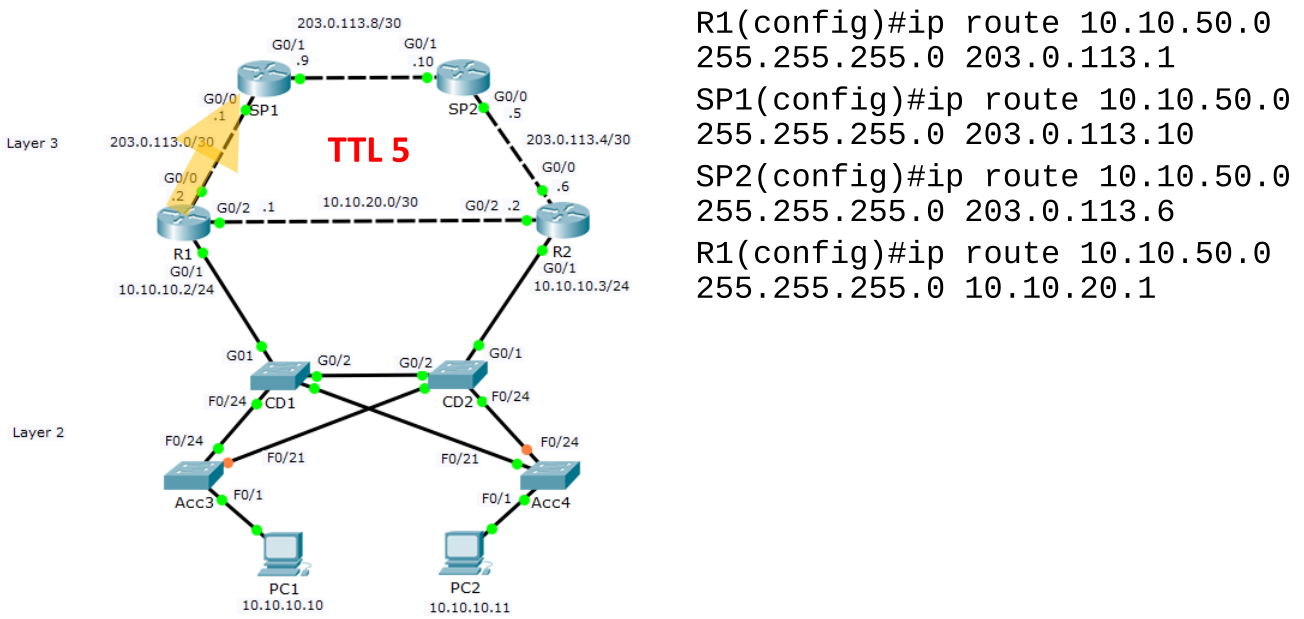
\includegraphics[width=\linewidth]{img/img17}
	\end{center}
\end{frame}

\begin{frame}{Routing Loop}
	\begin{center}
		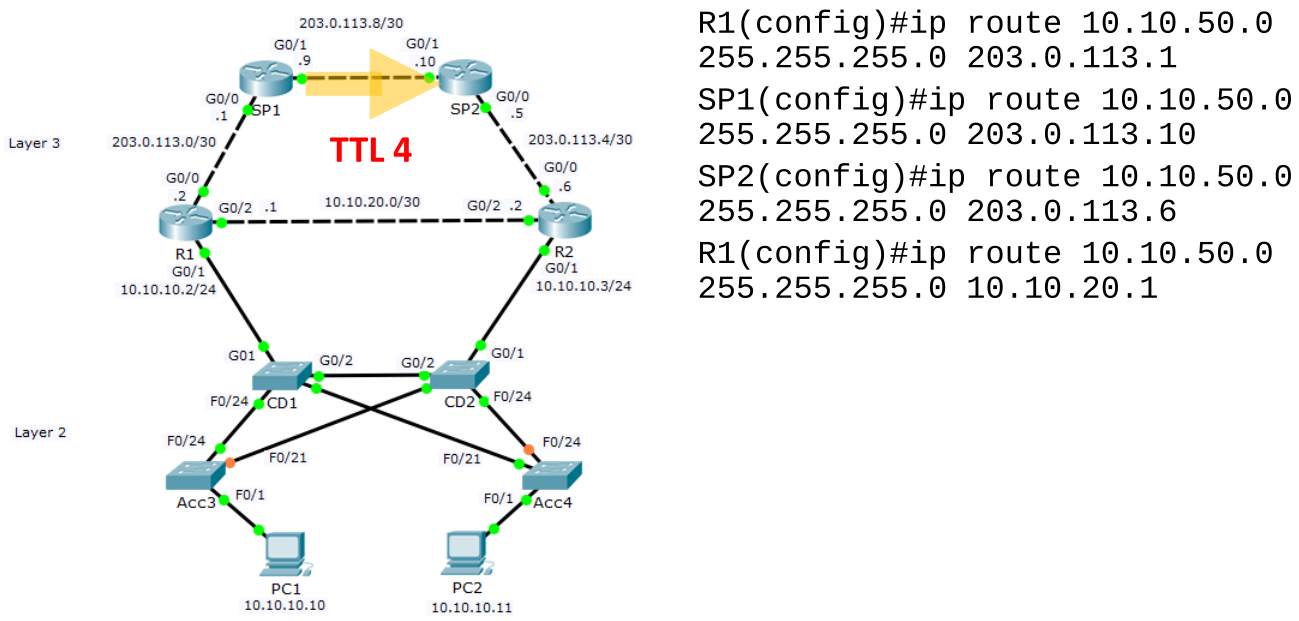
\includegraphics[width=\linewidth]{img/img18}
	\end{center}
\end{frame}

\begin{frame}{Routing Loop}
	\begin{center}
		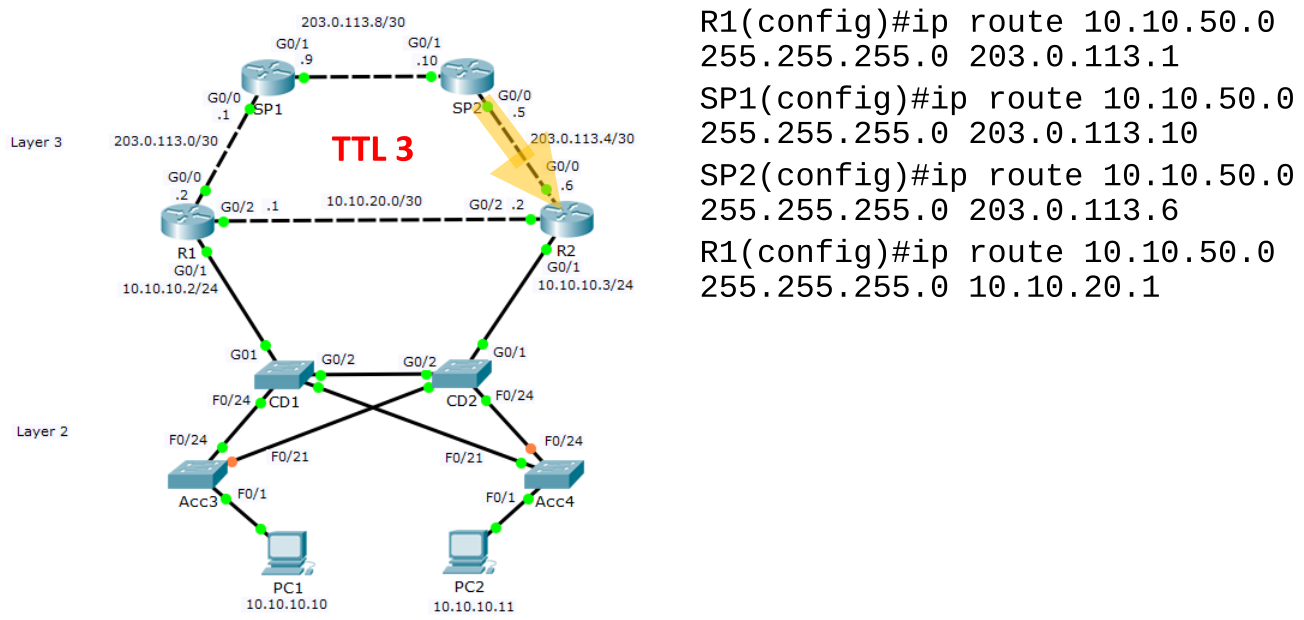
\includegraphics[width=\linewidth]{img/img19}
	\end{center}
\end{frame}

\begin{frame}{Routing Loop}
	\begin{center}
		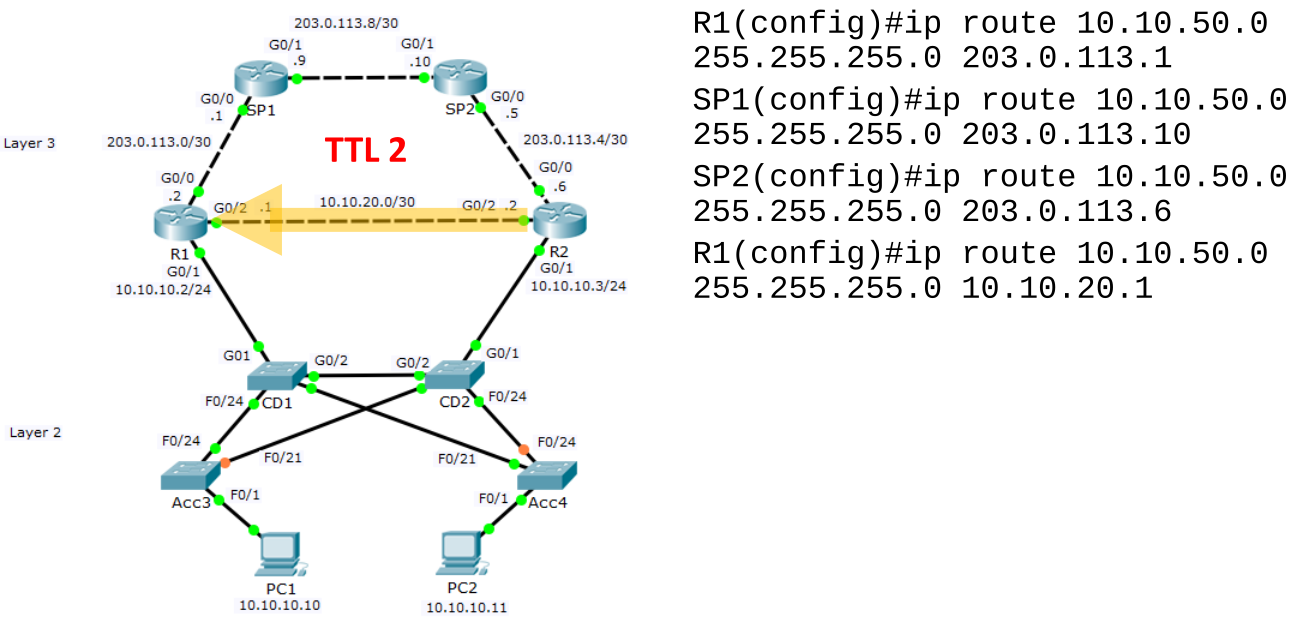
\includegraphics[width=\linewidth]{img/img20}
	\end{center}
\end{frame}

\begin{frame}{Routing Loop}
	\begin{center}
		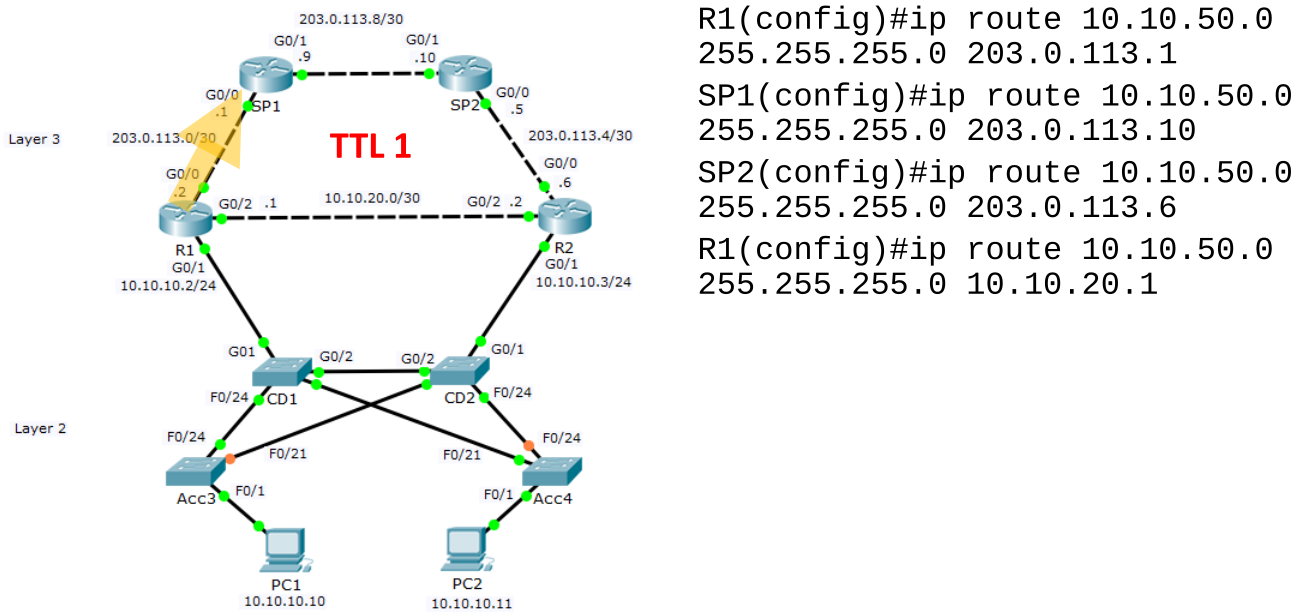
\includegraphics[width=\linewidth]{img/img21}
	\end{center}
\end{frame}

\begin{frame}
	\frametitle{ICMP Time Exceeded}
	\begin{center}
		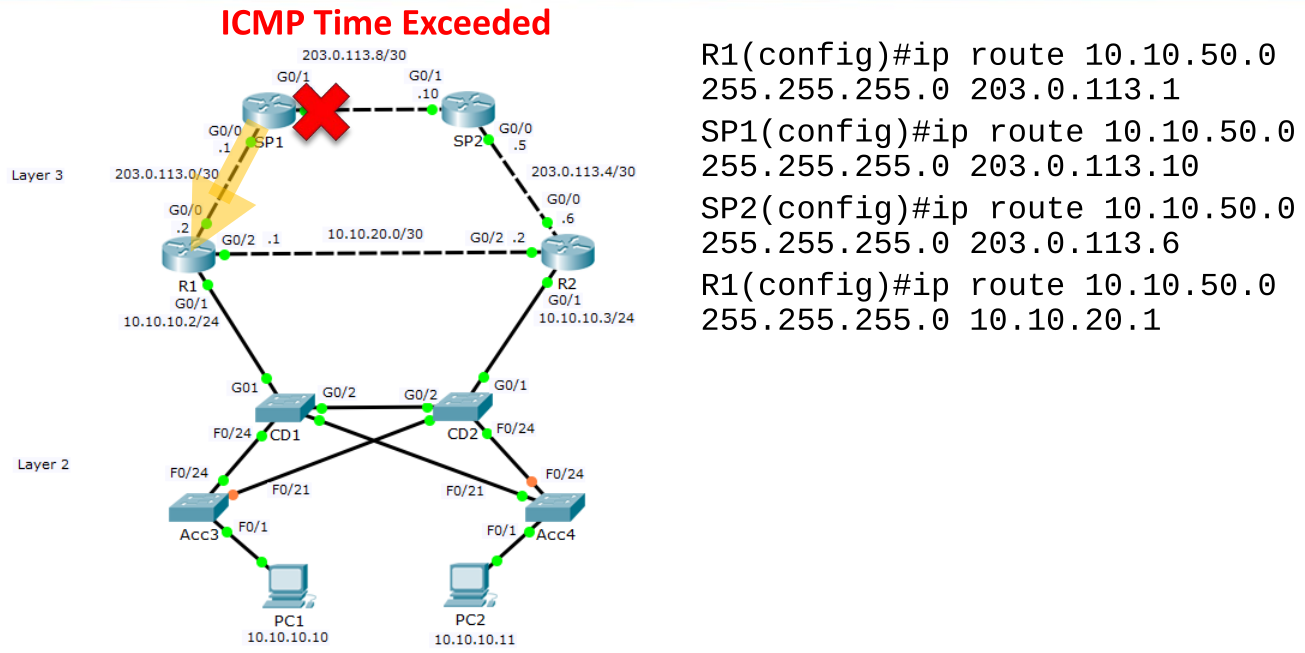
\includegraphics[width=\linewidth]{img/img22}
	\end{center}
\end{frame}

\begin{frame}
	\frametitle{Network Redundancy – Layer 3 Configuration}
	\begin{multicols}{2}
		\begin{center}
			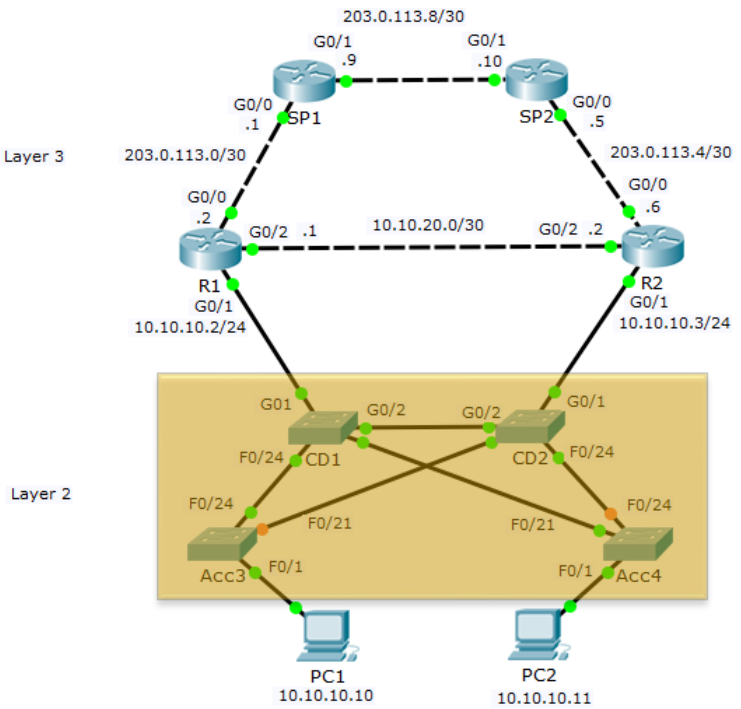
\includegraphics[width=\linewidth]{img/img23}
		\end{center}
		\columnbreak
		\begin{itemize}
			\item Layer 3 routing and HSRP will
control the path selection and
provide automatic failover for our
Layer 3 connections
			\item Dynamic routing protocols have
built-in loop prevention
mechanisms and TTL acts as a final
failsafe
			\item How will path selection, failover and
loop prevention work for the Layer 2
only switches?
		\end{itemize}
	\end{multicols}
\end{frame}

\section{Why we have the Spanning Tree Protocol}

\section{Spanning Tree Terminology - The Bridge}

\section{How Spanning Tree Works}

\section{Spanning Tree Versions}

\section{Verification - show spanning-tree}

\section{Verification - show mac address-table}

\section{Manipulating the Root Bridge Election}

\section{Spanning Tree and HSRP Alignment}

\section{Portfast, BPDU Guard and Root Guard}

\end{document}